%%%%%%%%%%%%%%%%%%%%%%%%%%%%%%%%%%%%%%%%%
% Beamer Presentation
% LaTeX Template
% Version 1.0 (10/11/12)
%
% This template has been downloaded from:
% http://www.LaTeXTemplates.com
%
% License:
% CC BY-NC-SA 3.0 (http://creativecommons.org/licenses/by-nc-sa/3.0/)
%
%%%%%%%%%%%%%%%%%%%%%%%%%%%%%%%%%%%%%%%%%

%----------------------------------------------------------------------------------------
%	PACKAGES AND THEMES
%----------------------------------------------------------------------------------------

\documentclass{beamer}
\usepackage[T1]{fontenc}
\usepackage{lmodern}
\usepackage[utf8]{inputenc}
\usepackage[german]{babel}
\usepackage[11pt]{moresize}


\mode<presentation> {

% The Beamer class comes with a number of default slide themes
% which change the colors and layouts of slides. Below this is a list
% of all the themes, uncomment each in turn to see what they look like.

%\usetheme{default}
%\usetheme{AnnArbor}
%\usetheme{Antibes}
%\usetheme{Bergen}
%\usetheme{Berkeley}
\usetheme{Berlin}
%\usetheme{Boadilla}
%\usetheme{CambridgeUS}
%\usetheme{Copenhagen}
%\usetheme{Darmstadt}
%\usetheme{Dresden}
%\usetheme{Frankfurt}
%\usetheme{Goettingen}
%\usetheme{Hannover}
%\usetheme{Ilmenau}
%\usetheme{JuanLesPins}
%\usetheme{Luebeck}
%\usetheme{Madrid}
%\usetheme{Malmoe}
%\usetheme{Marburg}
%\usetheme{Montpellier}
%\usetheme{PaloAlto}
%\usetheme{Pittsburgh}
%\usetheme{Rochester}
%\usetheme{Singapore}
%\usetheme{Szeged}
%\usetheme{Warsaw}

% As well as themes, the Beamer class has a number of color themes
% for any slide theme. Uncomment each of these in turn to see how it
% changes the colors of your current slide theme.

%\usecolortheme{albatross}
%\usecolortheme{beaver}
%\usecolortheme{beetle}
%\usecolortheme{crane}
%\usecolortheme{dolphin}
%\usecolortheme{dove}
%\usecolortheme{fly}
%\usecolortheme{lily}
%\usecolortheme{orchid}
%\usecolortheme{rose}
%\usecolortheme{seagull}
%\usecolortheme{seahorse}
%\usecolortheme{whale}
%\usecolortheme{wolverine}

%\setbeamertemplate{footline} % To remove the footer line in all slides uncomment this line
%\setbeamertemplate{footline}[page number] % To replace the footer line in all slides with a simple slide count uncomment this line

%\setbeamertemplate{navigation symbols}{} % To remove the navigation symbols from the bottom of all slides uncomment this line
}

\usepackage{graphicx} % Allows including images
\usepackage{booktabs} % Allows the use of \toprule, \midrule and \bottomrule in tables

%----------------------------------------------------------------------------------------
%	TITLE PAGE
%----------------------------------------------------------------------------------------

\title[Implementierungsphase]{Praxis der Softwareentwicklung\\ Implementierungsphase} % The short title appears at the bottom of every slide, the full title is only on the title page

\author{Phasenverantwortlicher: Pascal Zwick} % Your name
\institute[PSE] % Your institution as it will appear on the bottom of every slide, may be shorthand to save space
{

}
\date{05. Februar 2018} % Date, can be changed to a custom date

\begin{document}

\begin{frame}
\titlepage % Print the title page as the first slide
\end{frame}

%\begin{frame}
%\frametitle{Overview} % Table of contents slide, comment this block out to remove it
%\tableofcontents % Throughout your presentation, if you choose to use \section{} and \subsection{} commands, these will automatically be printed on this slide as an overview of your presentation
%\end{frame}

%----------------------------------------------------------------------------------------
%	PRESENTATION SLIDES
%----------------------------------------------------------------------------------------

%------------------------------------------------
\section{Zeitablauf} % Sections can be created in order to organize your presentation into discrete blocks, all sections and subsections are automatically printed in the table of contents as an overview of the talk
%------------------------------------------------
\begin{frame}
\frametitle{Gantt-Diagramm}
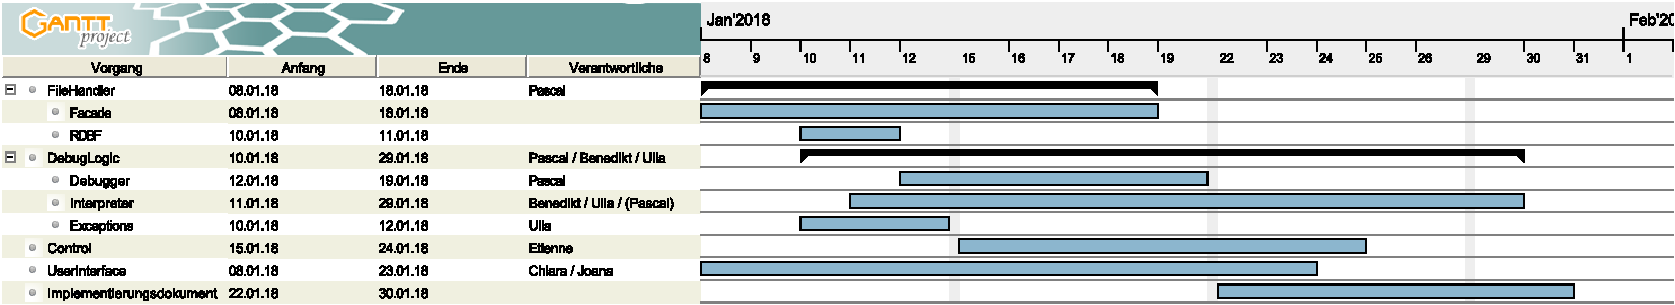
\includegraphics[scale=0.4]{../ganntDiagramm_neu_crop.pdf}
\end{frame}

\section{Nichtfunktionale-Anforderungen}
\subsection{Nichtfunktionale-Anforderungen}
\begin{frame}
\frametitle{Sicherstellung}
\begin{itemize}
\item Erweiterbarkeit: abstrakte Klassen und Schnittstellen (Interface)
\item Wartbarkeit: Javadoc, Kommentare im Quelltext und Nutzung von Checkstyle
\item Urheberrecht: GNU GPL 3 (GNU General Public License)
%\item Benutzerfreundlichkeit: NA
\end{itemize}
\end{frame}

\begin{frame}
\frametitle{Benutzerfreundlichkeit}
\begin{itemize}
\item Verständlichkeit: Sprachauswahl (Deutsch, Englisch)
\item Übersichtlichkeit: Simpel gehaltene Oberfläche
\item Erlernbarkeit: Hilfestellungen (Tooltips)
\item Modifizierbarkeit: Veränderung der Spaltengröße, ...
\end{itemize}
\end{frame}

\section{Entwurfsentscheidungen}
\subsection{Entwurfsmuster}
\begin{frame}
\frametitle{Singleton (Einzelstück)}
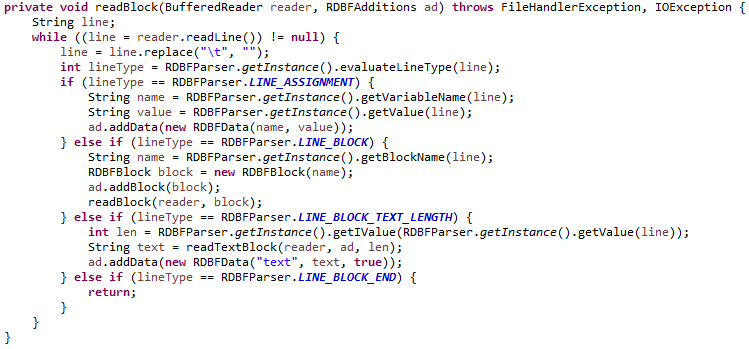
\includegraphics[scale=0.5]{../document_data/loadRDBFFile.png}
\end{frame}
\begin{frame}
\frametitle{Singleton (Einzelstück)}
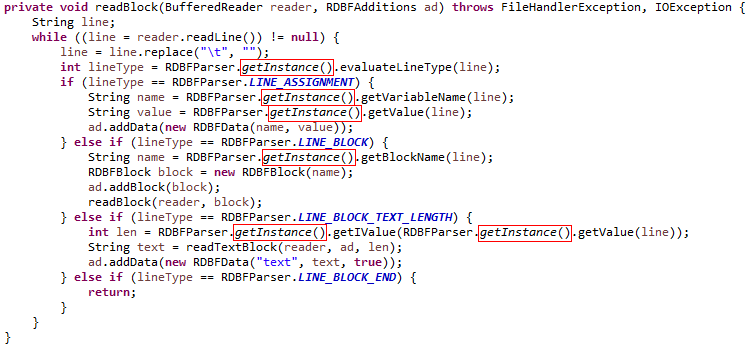
\includegraphics[scale=0.5]{../document_data/loadRDBFFile_instanceMarked.png}
\end{frame}

\begin{frame}
\frametitle{Strategy (Strategie)}
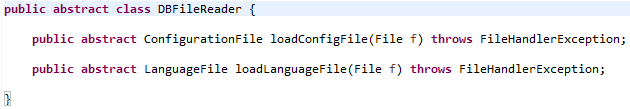
\includegraphics[scale=0.5]{../document_data/loadLangFileAbstract.png}
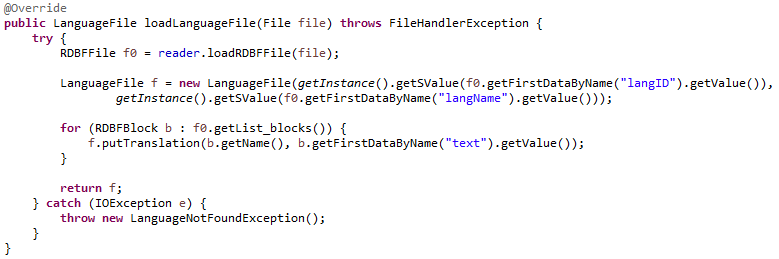
\includegraphics[scale=0.5]{../document_data/loadLangFile.png}
\end{frame}

\begin{frame}
\frametitle{Visitor (Besucher)}
\begin{itemize}
\item \textit{WlangBaseVisitor<T>}
\begin{itemize}
\item \textit{CommandGenerationVisitor}
\item \textit{TermGenerationVisitor}
\end{itemize}
\end{itemize}
\end{frame}

\begin{frame}
%\frametitle{While-Command}
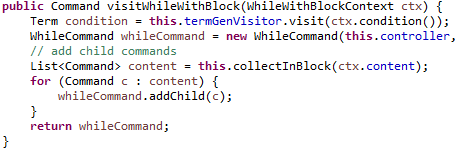
\includegraphics[scale=0.5]{../document_data/visitWhile.png}
\begin{itemize}
\item Kontext = Knoten (\textit{While-Knoten})
\item Besuchen der Bedingung
\item Sammeln und Hinzufügen der im \textit{while-block} stehenden Anweisungen
\end{itemize}
\end{frame}
\begin{frame}
%\frametitle{Terme (arithmetisch)}
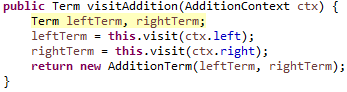
\includegraphics[scale=0.5]{../document_data/visitAddition.png}
\begin{itemize}
\item Besuchen beider Terme
\item Erstellen eines \textit{Addition} Terms, welcher beide Subterme enthält
\item Bsp: \textit{a = (b * c) + d}
\begin{itemize}
\item Linker Term: \textit{b * c}
\item Rechter Term: \textit{d}
\end{itemize}
\end{itemize}
\end{frame}

\subsection{Antlr}
\begin{frame}
\frametitle{Nutzung von Antlr}
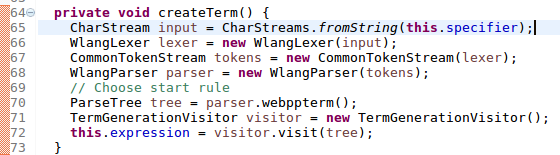
\includegraphics[scale=0.5]{../document_data/createTerm.png}
\begin{itemize}
\item Erzeugung eines Ableitungsbaums durch \textit{WlangLexer} und \textit{WlangParser}
\item \textit{Visitor} besuchen nun den generierten \textit{ParseTree}
\end{itemize}
\end{frame}

\begin{frame}
\frametitle{Commands (Befehle)}
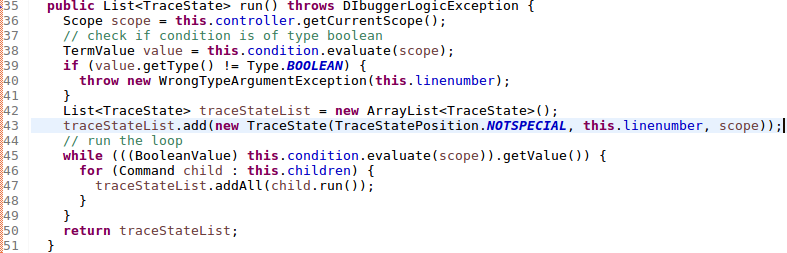
\includegraphics[scale=0.3]{../document_data/runWhile.png}
\begin{itemize}
\item Beispiel \textit{While-Command}
\item Holen des derzeitigen \textit{Scopes} (Stack-Frame)
\item Auswerten der \textit{Condition}
\item Befhle innerhalb der while-Schleife ausführen
\end{itemize}
\end{frame}

\section{Änderungen}
\subsection{FileHandler}
\begin{frame}
\frametitle{Exceptions Paket}
\begin{itemize}
\item Schnittstellen (Interface) können in Java nicht geworfen werden
\item \textit{FileHandlerException} wurde als abstrakte Klasse implementiert
\end{itemize}
\end{frame}

\subsection{DebugLogic}
\begin{frame}
\frametitle{Debugger und Interpreter}
\begin{itemize}
\item \textit{Subject} als Kontrollpunkt des Beobachtermusters
\item \textit{Observable} aus Java bietet gleiche Funktionalität
\item \textit{TraceIterator} bot Funktionalität zum iterieren über den Trace an
\item Trace wird in Form einer Liste gespeichert, also wurde \textit{ListIterator<T>} von Java benutzt
\end{itemize}
\end{frame}

\section{DIbugger}
%\subsection{DIbugger}
\begin{frame}
\frametitle{DIbugger}
\begin{center}

\includegraphics[scale=0.2]{../DIbugger/res/ui/logo_nongi.png}
\end{center}
\end{frame}

\end{document} 